\documentclass{standalone}
\usepackage{tikz}
\usepackage{ctex,mhchem}
\setCJKmainfont{Noto Serif CJK SC}
\usepackage{mhchem,siunitx}
\begin{document}
\small
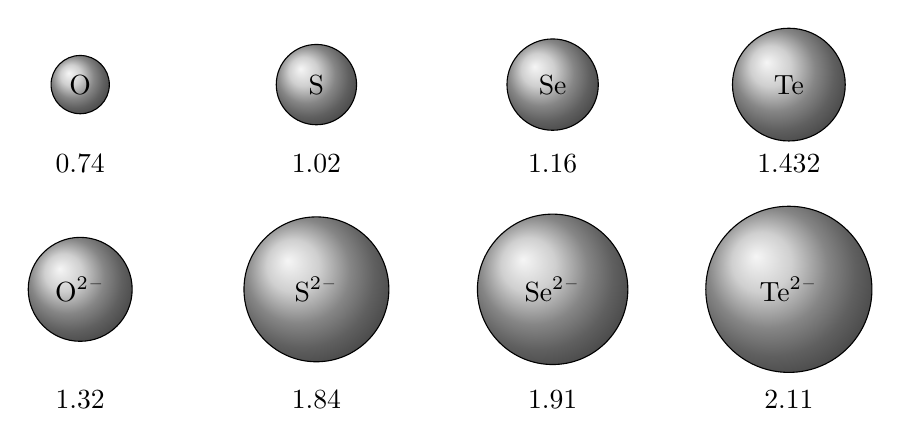
\begin{tikzpicture}[>=stealth]
  \foreach \x/\r/\R/\a in 
  {
    0/0.74/1.32/O,
    3/1.02/1.84/S,
    6/1.16/1.91/Se,
    9/1.432/2.11/Te%
    }
  {
    \draw[ball color= lightgray] (\x,1)circle(0.5*\r)node{\ce{\a}};
    \node at (\x,0){$\r$};
    \draw[ball color= lightgray] (\x,-1.6)circle(0.5*\R)node{\ce{{\a}^2-}};
    \node at (\x,-3){$\R$};
  }
\end{tikzpicture}
\end{document}